\documentclass[conference,a4paper]{IEEEtran}

\usepackage[spanish,es-tabla]{babel}
\usepackage[utf8]{inputenc}
\usepackage[T1]{fontenc}
\usepackage{graphicx}
\usepackage{booktabs}
\usepackage{array}
\usepackage{cite}
\usepackage{url}

\renewcommand{\abstractname}{Resumen}
\renewcommand{\IEEEkeywordsname}{Palabras clave}
\setlength{\textfloatsep}{6pt plus 1pt minus 2pt}
\setlength{\floatsep}{5pt plus 1pt minus 2pt}
\setlength{\intextsep}{5pt plus 1pt minus 2pt}
\setlength{\abovecaptionskip}{3pt}
\setlength{\belowcaptionskip}{0pt}

\title{Segmentaci\'on Sem\'antica y Control Aut\'onomo para un Veh\'iculo Robot con Jetson Nano}

\author{
\IEEEauthorblockN{Juan Jos\'e Prado Neira \quad Javier Rego Bargos}
\IEEEauthorblockA{Trabajo de Visi\'on Avanzada, TFM}
}

\begin{document}
\maketitle

\begin{abstract}
Este art\'iculo presenta una pr\'actica completa de visi\'on artificial aplicada a la conducci\'on aut\'onoma de un veh\'iculo robot basado en Jetson Nano. El sistema segmenta en tiempo real una zona transitable y obst\'aculos mediante una U-Net ligera entrenada con un conjunto de datos propio. La salida de la red se integra en una arquitectura distribuida donde la Jetson captura y aplica comandos, mientras que el port\'atil ejecuta la inferencia, calcula el desplazamiento lateral y genera las acciones de direcci\'on y velocidad. El modelo final alcanza un Dice de validaci\'on de 0.9519 y queda exportado a ONNX para su integraci\'on con OpenCV DNN u ONNX Runtime. La contribuci\'on principal es una cadena funcional que cubre anotaci\'on, entrenamiento, despliegue y control reactivo ante obst\'aculos.
\end{abstract}

\begin{IEEEkeywords}
visi\'on artificial, segmentaci\'on sem\'antica, U-Net, Jetson Nano, ONNX, rob\'otica m\'ovil.
\end{IEEEkeywords}

\section{Introducci\'on}
La conducci\'on aut\'onoma en plataformas rob\'oticas de bajo coste exige combinar percepci\'on visual, comunicaci\'on de baja latencia y control robusto. En este contexto, la segmentaci\'on sem\'antica resulta especialmente adecuada porque proporciona una descripci\'on densa de la escena: cada p\'ixel puede clasificarse como parte del circuito, obst\'aculo o fondo. Esta informaci\'on permite extraer una referencia geom\'etrica sencilla, como el centro de la zona transitable, sin depender de detectores de bordes fr\'agiles ni de reglas espec\'ificas para una iluminaci\'on concreta.

La pr\'actica desarrollada implementa un prototipo de extremo a extremo para un coche robot con Jetson Nano. El objetivo no es entrenar un modelo gen\'erico de conducci\'on, sino construir un sistema reproducible para seguir un circuito interior y reaccionar ante cajas situadas en la trayectoria. Para ello se crea un conjunto de datos propio, se entrena una U-Net compacta de dos salidas y se integra el modelo en un flujo distribuido de v\'ideo y control. Esta separaci\'on permite ejecutar en el port\'atil el c\'omputo pesado de inferencia, manteniendo en la Jetson la captura de c\'amara y la aplicaci\'on final de los comandos al veh\'iculo.

\section{Metodolog\'ia}
El flujo de trabajo se dividi\'o en cuatro etapas: adquisici\'on de datos, entrenamiento, exportaci\'on del modelo e integraci\'on con el sistema de control. Primero se capturaron im\'agenes reales del circuito desde una perspectiva baja, similar a la del veh\'iculo. Las muestras se anotaron con MakeSense en dos clases: \texttt{circuito}, que representa la zona transitable, y \texttt{caja}, que representa obst\'aculos. A partir del fichero COCO exportado se generaron m\'ascaras binarias independientes para cada clase.

El flujo de entrenamiento toma como referencia la pr\'actica DeepLabv3+ del Tema 5~\cite{practica5}, centrada en dataloaders, Dice+BCE e IoU para segmentaci\'on sem\'antica, y los fundamentos DeepLabv3/v3+~\cite{deeplabv3,deeplabv3plus}. Para este prototipo se eligi\'o una U-Net ligera, inspirada en la arquitectura encoder--decoder con conexiones de salto propuesta por Ronneberger \textit{et al.}~\cite{ronneberger2015unet}. La red recibe una imagen RGB de $256 \times 256$ p\'ixeles y produce dos mapas de logits: circuito y obst\'aculos. El entrenamiento se realiz\'o en PyTorch con Adam y una p\'erdida BCEWithLogits + Dice Loss ponderada para la clase de obst\'aculo.

La salida entrenada se export\'o a ONNX para separar el entrenamiento del entorno de ejecuci\'on. En el runtime de visi\'on, el modelo puede cargarse con OpenCV DNN y, si ese backend falla, con ONNX Runtime. Tras la inferencia se aplica una sigmoide por canal, umbrales configurables y operaciones morfol\'ogicas sobre la m\'ascara del circuito. El centro de la zona transitable se calcula en una regi\'on de inter\'es inferior de la imagen, donde la perspectiva del veh\'iculo proporciona la informaci\'on m\'as relevante para la direcci\'on inmediata.

\section{Arquitectura del Sistema}
El sistema completo est\'a organizado en cuatro bloques de software. El m\'odulo \texttt{vision} procesa cada frame, ejecuta la segmentaci\'on y construye la informaci\'on de carril. El m\'odulo \texttt{conexion} implementa el transporte de v\'ideo, el receptor local y la orquestaci\'on del arranque remoto. El m\'odulo \texttt{control} define el protocolo de comandos y el cliente de control manual. Finalmente, \texttt{jetson} contiene los procesos remotos que capturan la c\'amara y aplican las \'ordenes al veh\'iculo.

Durante la ejecuci\'on, la Jetson env\'ia frames JPEG al port\'atil mediante UDP. La configuraci\'on del repositorio fija una resoluci\'on de captura de $512 \times 288$ y una frecuencia objetivo de 12 FPS. El receptor decodifica cada imagen, obtiene las m\'ascaras, suaviza el desplazamiento lateral con una media exponencial y calcula una acci\'on autom\'atica normalizada. La orden se devuelve a la Jetson como un mensaje JSON por l\'inea con los campos \textit{steering}, \textit{throttle}, modo y raz\'on de la decisi\'on.

\begin{table}[t]
\centering
\caption{Resumen t\'ecnico del sistema desarrollado.}
\label{tab:resumen}
\footnotesize
\begin{tabular}{@{}p{0.42\linewidth}p{0.50\linewidth}@{}}
\toprule
\textbf{Elemento} & \textbf{Valor} \\
\midrule
Dataset & 57 im\'agenes, 100 anotaciones \\
Clases & \texttt{circuito}, \texttt{caja} \\
Resoluci\'on original & $640 \times 360$ p\'ixeles \\
Partici\'on & 45 entrenamiento, 12 validaci\'on \\
Modelo & U-Net ligera, 7.763.074 par\'ametros \\
Entrada / salida & $3 \times 256 \times 256$ / $2 \times 256 \times 256$ \\
Optimizador & Adam, \textit{batch size} 8 \\
P\'erdida & BCEWithLogits + Dice Loss \\
Mejor checkpoint & \'Epoca 78, Dice 0.9519 \\
Despliegue & ONNX con OpenCV DNN/ONNX Runtime \\
Control & \textit{steering}, \textit{throttle}, parada/evas\'ion \\
\bottomrule
\end{tabular}
\end{table}

La pol\'itica de autonom\'ia combina seguimiento de circuito y evitaci\'on de obst\'aculos. Si existe centro de carril, el error lateral se normaliza respecto a la mitad del ancho de la imagen y se transforma en direcci\'on mediante una ganancia proporcional y un t\'ermino de curvatura. Cuando la m\'ascara de obst\'aculo supera umbrales de \'area y tama\~no dentro de la regi\'on frontal, el sistema decide entre reducir velocidad, rodear el obst\'aculo o detenerse. Si se pierde el centro del circuito, la pol\'itica configurada detiene el veh\'iculo para evitar acciones ciegas.

\section{Resultados}
El entrenamiento produjo un checkpoint seleccionado por Dice de validaci\'on. El mejor modelo se guard\'o en la \'epoca 78 con un Dice de 0.9519, lo que indica alta coincidencia entre las m\'ascaras predichas y las anotaciones de validaci\'on. La m\'etrica debe interpretarse dentro del alcance del conjunto de datos: se trata de un escenario controlado, con 57 im\'agenes y una divisi\'on de validaci\'on de 12 muestras. Por tanto, el resultado confirma la viabilidad de la pr\'actica, pero no sustituye una evaluaci\'on en circuitos, c\'amaras e iluminaciones no vistas.

\begin{figure}[t]
\centering
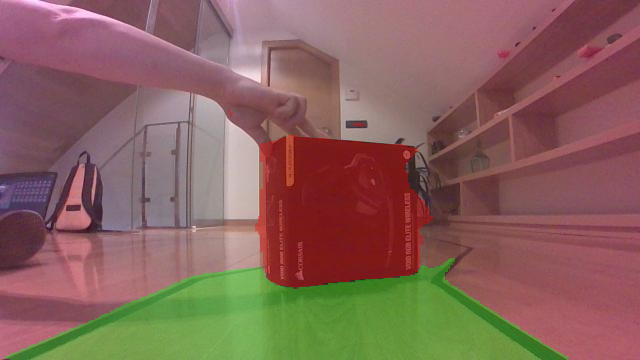
\includegraphics[width=\linewidth]{../circuito_segmentation/outputs/revision_lote/50_prediction.png}
\caption{Ejemplo de inferencia: zona transitable segmentada en verde y obst\'aculo en rojo.}
\label{fig:prediccion}
\end{figure}

La Fig.~\ref{fig:prediccion} muestra una predicci\'on representativa del sistema. La m\'ascara verde proporciona la referencia para calcular el centro de la trayectoria y la m\'ascara roja activa la l\'ogica de precauci\'on ante obst\'aculos. El uso de una salida multicanal facilita que ambas decisiones procedan de una misma pasada de inferencia, lo que simplifica la sincronizaci\'on entre percepci\'on y control. Adem\'as, el postprocesado morfol\'ogico reduce peque\~nas discontinuidades en la m\'ascara del circuito antes de extraer el centro.

En la integraci\'on, el sistema queda preparado para operar con arranque coordinado desde el port\'atil. El script principal sincroniza los componentes necesarios en la Jetson, inicia el emisor de v\'ideo, levanta el servidor de control remoto y abre el receptor local con la interfaz de visi\'on. Esta organizaci\'on permiti\'o aislar responsabilidades: la Jetson conserva la interacci\'on con hardware y el port\'atil concentra la inferencia y la depuraci\'on visual. No se registraron en el repositorio medidas experimentales cerradas de latencia o FPS real, por lo que esos valores se documentan como configuraci\'on objetivo y no como resultado medido.

\section{Discusi\'on}
El enfoque es adecuado para rob\'otica educativa porque la segmentaci\'on sem\'antica ofrece una se\~nal de control interpretable: las m\'ascaras pueden visualizarse y compararse con anotaciones. ONNX desacopla entrenamiento y despliegue, mientras que el reparto Jetson--port\'atil reduce la carga embebida. Las principales limitaciones son el tama\~no del dataset y la dependencia del entorno: la red podr\'ia degradarse ante suelos, brillos, c\'amaras o posiciones de obst\'aculos no vistas. Queda pendiente medir latencia extremo a extremo, FPS real, estabilidad del seguimiento e intervenciones manuales por vuelta.

\section{Conclusiones}
Se ha desarrollado un sistema funcional de percepci\'on y control para un veh\'iculo robot con Jetson Nano. La soluci\'on integra un dataset propio, una U-Net ligera de dos canales, exportaci\'on ONNX y un runtime distribuido que transforma m\'ascaras en comandos de \textit{steering} y \textit{throttle}. El Dice de validaci\'on de 0.9519 confirma la viabilidad del enfoque en el escenario planteado. Como trabajo futuro se propone ampliar datos, optimizar con TensorRT y medir latencia, FPS y robustez.

\begin{thebibliography}{1}
\bibitem{practica5}
Material docente de Visi\'on Avanzada, ``Segmentaci\'on con DeepLabv3+,'' Tema 5, 2026.

\bibitem{deeplabv3}
L.-C.~Chen, G.~Papandreou, F.~Schroff y H.~Adam, ``Rethinking Atrous Convolution for Semantic Image Segmentation,'' arXiv:1706.05587, 2017.

\bibitem{deeplabv3plus}
L.-C.~Chen, Y.~Zhu, G.~Papandreou, F.~Schroff y H.~Adam, ``Encoder-Decoder with Atrous Separable Convolution for Semantic Image Segmentation,'' en \textit{ECCV}, 2018.

\bibitem{ronneberger2015unet}
O.~Ronneberger, P.~Fischer y T.~Brox, ``U-Net: Convolutional Networks for Biomedical Image Segmentation,'' en \textit{MICCAI}, 2015.

\bibitem{pytorch}
A.~Paszke \textit{et al.}, ``PyTorch: An Imperative Style, High-Performance Deep Learning Library,'' en \textit{NeurIPS}, 2019.

\end{thebibliography}

\end{document}
